%----------------------------------------------------------------------------------------
%    PACKAGES AND THEMES
%----------------------------------------------------------------------------------------
\documentclass[aspectratio=169,xcolor=dvipsnames]{beamer}
\makeatletter
\def\input@path{{../BeamerTemplate/theme/}}
\makeatother
\usetheme{CleanEasy}
\usepackage[utf8]{inputenc}
\usepackage{lmodern}
\usepackage[T1]{fontenc}
\usepackage{fix-cm}
\usepackage{amsmath}
\usepackage{mathtools}
\usepackage{listings}
\usepackage{xcolor}
\usepackage{hyperref}
\usepackage{graphicx}
\usepackage{booktabs}
\usepackage{tikz}
\usetikzlibrary{positioning, shapes, arrows, calc, decorations.pathreplacing, arrows.meta, backgrounds, patterns, overlay-beamer-styles}
\usepackage{etoolbox}
\usepackage{animate}

%----------------------------------------------------------------------------------------
%    LAYOUT CONFIGURATION
%----------------------------------------------------------------------------------------
\input{../BeamerTemplate/configs/configs}

%----------------------------------------------------------------------------------------
%    TITLE PAGE CONFIGURATION
%----------------------------------------------------------------------------------------
\title[Queues]{Data Structures: Queues}
\author{Minseok Jeon}
\institute{DGIST}
\date{\today}

% Simple title page without logos
\titlegraphic{}

%----------------------------------------------------------------------------------------

\begin{document}

\begin{frame}[plain]
  \titlepage
\end{frame}

\begin{frame}[plain]{Contents}
  \tableofcontents
\end{frame}

%----------------------------------------------------------------------------------------
%    INTRODUCTION
%----------------------------------------------------------------------------------------
\section{Introduction to Queues}

\begin{frame}{What is a Queue?}
  \begin{definition}
    A \textbf{queue} is a linear data structure that follows the \textbf{First In, First Out (FIFO)} principle.
  \end{definition}

  \vspace{0.5cm}

  \begin{columns}
    \begin{column}{0.6\textwidth}
      Key characteristics:
      \begin{itemize}
        \item Elements are inserted at the rear (enqueue)
        \item Elements are removed from the front (dequeue)
        \item Perfect for scheduling and buffering
        \item Models real-world waiting lines
        \item Used in OS scheduling and network packet handling
      \end{itemize}
    \end{column}
    \begin{column}{0.35\textwidth}
      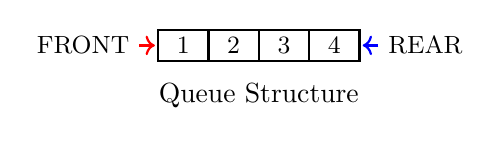
\begin{tikzpicture}[scale=0.8]
        % Queue representation
        \draw[thick] (0,0.5) rectangle (0.8,1);
        \draw[thick] (0.8,0.5) rectangle (1.6,1);
        \draw[thick] (1.6,0.5) rectangle (2.4,1);
        \draw[thick] (2.4,0.5) rectangle (3.2,1);

        \node at (0.4,0.75) {\small 1};
        \node at (1.2,0.75) {\small 2};
        \node at (2.0,0.75) {\small 3};
        \node at (2.8,0.75) {\small 4};

        % Front arrow
        \draw[->, thick, red] (-0.3,0.75) -- (-0.05,0.75);
        \node[left] at (-0.3,0.75) {\small FRONT};

        % Rear arrow
        \draw[->, thick, blue] (3.5,0.75) -- (3.25,0.75);
        \node[right] at (3.5,0.75) {\small REAR};

        \node[below] at (1.6,0.3) {Queue Structure};
      \end{tikzpicture}
    \end{column}
  \end{columns}
\end{frame}

%----------------------------------------------------------------------------------------
%    CORE OPERATIONS
%----------------------------------------------------------------------------------------
\section{Core Operations}

\begin{frame}[fragile]{Essential Queue Operations}
  \begin{columns}
    \begin{column}{0.5\textwidth}
      \begin{block}{Primary Operations}
        \begin{itemize}
          \item \textbf{Enqueue}: Add element to rear
          \item \textbf{Dequeue}: Remove and return front element
          \item \textbf{Front/Peek}: View front element without removing
          \item \textbf{Empty}: Check if queue is empty
          \item \textbf{Size}: Get number of elements
        \end{itemize}
      \end{block}
    \end{column}
    \begin{column}{0.45\textwidth}
      \begin{exampleblock}{C Example}
        \begin{lstlisting}[language=C,basicstyle=\tiny\ttfamily]
#include <stdio.h>
#include <stdlib.h>

typedef struct Node {
    int data;
    struct Node* next;
} Node;

typedef struct Queue {
    Node *front, *rear;
} Queue;

void enqueue(Queue* q, int x) {
    Node* n = malloc(sizeof(Node));
    n->data = x; n->next = NULL;
    if (q->rear) q->rear->next = n;
    q->rear = n;
    if (!q->front) q->front = n;
}

int dequeue(Queue* q) {
    int x = q->front->data;
    Node* tmp = q->front;
    q->front = q->front->next;
    if (!q->front) q->rear = NULL;
    free(tmp); return x;
}

int isEmpty(Queue* q) {
    return q->front == NULL;
}
        \end{lstlisting}
      \end{exampleblock}
    \end{column}
  \end{columns}

  \vspace{0.5cm}

  \begin{alertblock}{Time Complexity}
    All operations are \textbf{O(1)} - constant time
  \end{alertblock}
\end{frame}

\begin{frame}{Queue Operations Visualization}
  \begin{center}
    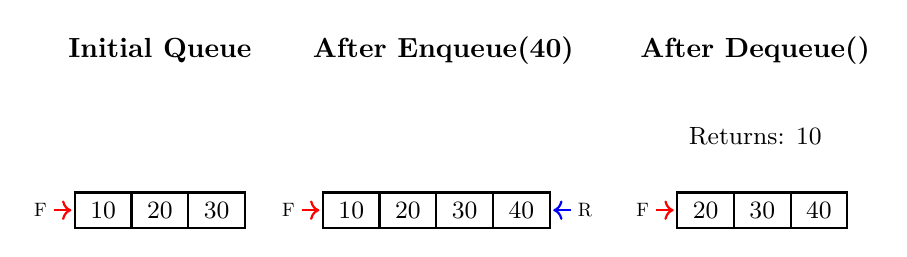
\begin{tikzpicture}[scale=0.9]
      % Initial queue
      \node at (1.2,3) {\textbf{Initial Queue}};
      \draw[thick] (0,0.5) rectangle (0.8,1);
      \draw[thick] (0.8,0.5) rectangle (1.6,1);
      \draw[thick] (1.6,0.5) rectangle (2.4,1);
      \node at (0.4,0.75) {\small 10};
      \node at (1.2,0.75) {\small 20};
      \node at (2.0,0.75) {\small 30};
      \draw[->, thick, red] (-0.3,0.75) -- (-0.05,0.75);
      \node[left, scale=0.7] at (-0.3,0.75) {F};

      % After Enqueue(40)
      \node at (5.2,3) {\textbf{After Enqueue(40)}};
      \draw[thick] (3.5,0.5) rectangle (4.3,1);
      \draw[thick] (4.3,0.5) rectangle (5.1,1);
      \draw[thick] (5.1,0.5) rectangle (5.9,1);
      \draw[thick] (5.9,0.5) rectangle (6.7,1);
      \node at (3.9,0.75) {\small 10};
      \node at (4.7,0.75) {\small 20};
      \node at (5.5,0.75) {\small 30};
      \node at (6.3,0.75) {\small 40};
      \draw[->, thick, red] (3.2,0.75) -- (3.45,0.75);
      \node[left, scale=0.7] at (3.2,0.75) {F};
      \draw[->, thick, blue] (7.0,0.75) -- (6.75,0.75);
      \node[right, scale=0.7] at (7.0,0.75) {R};

      % After Dequeue()
      \node at (9.6,3) {\textbf{After Dequeue()}};
      \draw[thick] (8.5,0.5) rectangle (9.3,1);
      \draw[thick] (9.3,0.5) rectangle (10.1,1);
      \draw[thick] (10.1,0.5) rectangle (10.9,1);
      \node at (8.9,0.75) {\small 20};
      \node at (9.7,0.75) {\small 30};
      \node at (10.5,0.75) {\small 40};
      \draw[->, thick, red] (8.2,0.75) -- (8.45,0.75);
      \node[left, scale=0.7] at (8.2,0.75) {F};

      \node at (9.6,1.8) {\small Returns: 10};
    \end{tikzpicture}
  \end{center}
\end{frame}

%----------------------------------------------------------------------------------------
%    CIRCULAR QUEUE
%----------------------------------------------------------------------------------------
\section{Circular Queue}

\begin{frame}{Circular Queue Concept}
  \begin{columns}
    \begin{column}{0.55\textwidth}
      \begin{block}{Why Circular Queue?}
        \begin{itemize}
          \item Simple array queue wastes space
          \item Front pointer moves forward
          \item Space at beginning becomes unusable
          \item Solution: Wrap around using modulo
        \end{itemize}
      \end{block}

      \begin{alertblock}{Wrap-around Formula}
        \texttt{(index + 1) \% capacity}
      \end{alertblock}

      \textbf{Full/Empty Detection:}
      \begin{itemize}
        \item Track size explicitly, OR
        \item Reserve one empty slot
      \end{itemize}
    \end{column}
    \begin{column}{0.4\textwidth}
      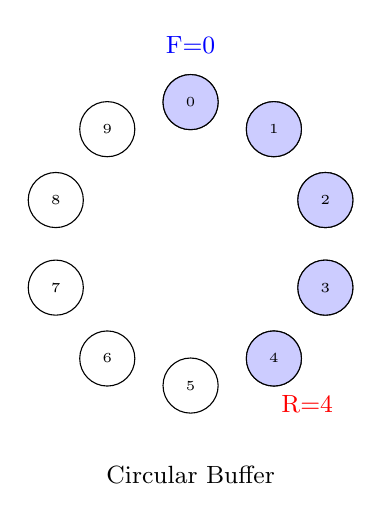
\begin{tikzpicture}[scale=0.9]
        % Circular array
        \foreach \angle/\num in {90/0, 54/1, 18/2, -18/3, -54/4, -90/5, -126/6, -162/7, 162/8, 126/9} {
          \node[circle, draw, minimum size=0.7cm] (n\num) at (\angle:2cm) {\tiny \num};
        }

        % Front and rear markers
        \node[blue, font=\small] at (90:2.8cm) {F=0};
        \node[red, font=\small] at (-54:2.8cm) {R=4};

        % Show some filled elements
        \node[circle, draw, fill=blue!20, minimum size=0.7cm] at (90:2cm) {\tiny 0};
        \node[circle, draw, fill=blue!20, minimum size=0.7cm] at (54:2cm) {\tiny 1};
        \node[circle, draw, fill=blue!20, minimum size=0.7cm] at (18:2cm) {\tiny 2};
        \node[circle, draw, fill=blue!20, minimum size=0.7cm] at (-18:2cm) {\tiny 3};
        \node[circle, draw, fill=blue!20, minimum size=0.7cm] at (-54:2cm) {\tiny 4};

        \node[below] at (0,-3) {\small Circular Buffer};
      \end{tikzpicture}
    \end{column}
  \end{columns}
\end{frame}

\begin{frame}[fragile]{Circular Queue Implementation}
  \begin{lstlisting}[language=Python,basicstyle=\small\ttfamily]
class CircularQueue:
    def __init__(self, capacity):
        self.data = [None] * capacity
        self.capacity = capacity
        self.front = 0
        self.size = 0

    def enqueue(self, item):
        if self.size == self.capacity:
            raise Exception("Queue is full")
        rear = (self.front + self.size) % self.capacity
        self.data[rear] = item
        self.size += 1

    def dequeue(self):
        if self.size == 0:
            raise Exception("Queue is empty")
        item = self.data[self.front]
        self.front = (self.front + 1) % self.capacity
        self.size -= 1
        return item
  \end{lstlisting}
\end{frame}

%----------------------------------------------------------------------------------------
%    DEQUE
%----------------------------------------------------------------------------------------
\section{Deque (Double-Ended Queue)}

\begin{frame}{Deque: Double-Ended Queue}
  \begin{definition}
    A \textbf{deque} (pronounced "deck") allows insertion and deletion at both ends.
  \end{definition}

  \vspace{0.3cm}

  \begin{columns}
    \begin{column}{0.55\textwidth}
      \begin{block}{Deque Operations}
        \begin{itemize}
          \item \texttt{pushFront(x)}: Insert at front
          \item \texttt{pushBack(x)}: Insert at rear
          \item \texttt{popFront()}: Remove from front
          \item \texttt{popBack()}: Remove from rear
        \end{itemize}
      \end{block}

      \begin{exampleblock}{Use Cases}
        \begin{itemize}
          \item Palindrome checking
          \item Sliding window algorithms
          \item Browser history (forward/back)
          \item Undo/redo with priorities
        \end{itemize}
      \end{exampleblock}
    \end{column}
    \begin{column}{0.4\textwidth}
      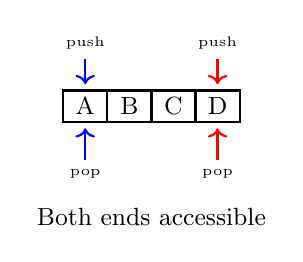
\begin{tikzpicture}[scale=0.8]
        % Deque representation
        \draw[thick] (0,1) rectangle (0.7,1.5);
        \draw[thick] (0.7,1) rectangle (1.4,1.5);
        \draw[thick] (1.4,1) rectangle (2.1,1.5);
        \draw[thick] (2.1,1) rectangle (2.8,1.5);

        \node at (0.35,1.25) {\small A};
        \node at (1.05,1.25) {\small B};
        \node at (1.75,1.25) {\small C};
        \node at (2.45,1.25) {\small D};

        % Operations arrows
        \draw[->, thick, blue] (0.35,2) -- (0.35,1.6);
        \node[above] at (0.35,2) {\tiny push};
        \draw[->, thick, blue] (0.35,0.4) -- (0.35,0.9);
        \node[below] at (0.35,0.4) {\tiny pop};

        \draw[->, thick, red] (2.45,2) -- (2.45,1.6);
        \node[above] at (2.45,2) {\tiny push};
        \draw[->, thick, red] (2.45,0.4) -- (2.45,0.9);
        \node[below] at (2.45,0.4) {\tiny pop};

        \node at (1.4,-0.5) {\small Both ends accessible};
      \end{tikzpicture}
    \end{column}
  \end{columns}
\end{frame}

%----------------------------------------------------------------------------------------
%    PRIORITY QUEUE
%----------------------------------------------------------------------------------------
\section{Priority Queue}

\begin{frame}{Priority Queue}
  \begin{definition}
    A \textbf{priority queue} is a queue where elements are served based on priority rather than insertion order.
  \end{definition}

  \vspace{0.3cm}

  \begin{columns}
    \begin{column}{0.5\textwidth}
      \begin{block}{Key Properties}
        \begin{itemize}
          \item Each element has a priority
          \item Highest (or lowest) priority served first
          \item Typically implemented with binary heap
          \item Insert: O(log n)
          \item Extract-min/max: O(log n)
          \item Peek: O(1)
        \end{itemize}
      \end{block}
    \end{column}
    \begin{column}{0.45\textwidth}
      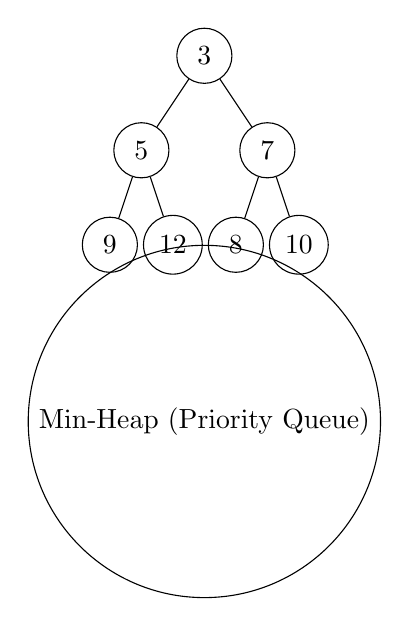
\begin{tikzpicture}[scale=0.8,
        level 1/.style={sibling distance=20mm},
        level 2/.style={sibling distance=10mm},
        every node/.style={circle, draw, minimum size=7mm}]
        \node {3}
          child {node {5}
            child {node {9}}
            child {node {12}}
          }
          child {node {7}
            child {node {8}}
            child {node {10}}
          };
        \node[below] at (0,-3) {Min-Heap (Priority Queue)};
      \end{tikzpicture}

      \vspace{0.3cm}
      \begin{alertblock}{Applications}
        Dijkstra's algorithm, task scheduling, event simulation
      \end{alertblock}
    \end{column}
  \end{columns}
\end{frame}

%----------------------------------------------------------------------------------------
%    IMPLEMENTATIONS
%----------------------------------------------------------------------------------------
\section{Implementation Approaches}

\begin{frame}{Array-based vs Linked List Implementation}
  \begin{center}
    \begin{tabular}{l|c|c}
      \toprule
      \textbf{Feature} & \textbf{Array-based} & \textbf{Linked List-based} \\
      \midrule
      Time Complexity & O(1) amortized & O(1) guaranteed \\
      Space Efficiency & Better (contiguous) & More overhead (pointers) \\
      Cache Performance & Excellent & Fair \\
      Resize Cost & Occasional O(n) & Never \\
      Capacity & Fixed (or resizable) & Dynamic \\
      \bottomrule
    \end{tabular}
  \end{center}

  \vspace{0.5cm}

  \begin{columns}
    \begin{column}{0.48\textwidth}
      \begin{block}{Array-based Queue}
        \begin{itemize}
          \item Use circular buffer
          \item Track front and rear indices
          \item Better for bounded queues
        \end{itemize}
      \end{block}
    \end{column}
    \begin{column}{0.48\textwidth}
      \begin{block}{Linked List Queue}
        \begin{itemize}
          \item Maintain front and rear pointers
          \item No capacity concerns
          \item Better for unbounded queues
        \end{itemize}
      \end{block}
    \end{column}
  \end{columns}
\end{frame}

\begin{frame}[fragile]{Linked List Queue Implementation}
  \begin{lstlisting}[language=Python,basicstyle=\small\ttfamily]
class Node:
    def __init__(self, val, next=None):
        self.val = val
        self.next = next

class QueueLL:
    def __init__(self):
        self.front = None
        self.rear = None
        self.size = 0

    def enqueue(self, x):
        new_node = Node(x)
        if self.rear:
            self.rear.next = new_node
        self.rear = new_node
        if not self.front:
            self.front = new_node
        self.size += 1

    def dequeue(self):
        if not self.front:
            raise Exception("Queue is empty")
        val = self.front.val
        self.front = self.front.next
        if not self.front:
            self.rear = None
        self.size -= 1
        return val
  \end{lstlisting}
\end{frame}

%----------------------------------------------------------------------------------------
%    APPLICATIONS
%----------------------------------------------------------------------------------------
\section{Applications}

\begin{frame}{Producer-Consumer Pattern}
  \begin{columns}
    \begin{column}{0.55\textwidth}
      \begin{block}{Bounded Buffer Problem}
        \begin{itemize}
          \item Producers generate data
          \item Consumers process data
          \item Queue acts as buffer
          \item Handles rate mismatch
        \end{itemize}
      \end{block}

      \textbf{Synchronization:}
      \begin{itemize}
        \item If full → producer waits
        \item If empty → consumer waits
        \item Use locks/semaphores for thread safety
      \end{itemize}
    \end{column}
    \begin{column}{0.4\textwidth}
      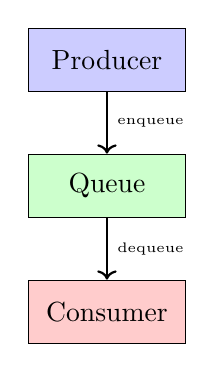
\begin{tikzpicture}[scale=0.8,
        block/.style={rectangle, draw, minimum width=2cm, minimum height=0.8cm}]

        \node[block, fill=blue!20] (prod) at (0,2) {Producer};
        \node[block, fill=green!20] (queue) at (0,0) {Queue};
        \node[block, fill=red!20] (cons) at (0,-2) {Consumer};

        \draw[->, thick] (prod) -- (queue) node[midway,right] {\tiny enqueue};
        \draw[->, thick] (queue) -- (cons) node[midway,right] {\tiny dequeue};
      \end{tikzpicture}

      \vspace{0.3cm}
      \begin{exampleblock}{Examples}
        Print spooler, web server request handling
      \end{exampleblock}
    \end{column}
  \end{columns}
\end{frame}

\begin{frame}{Queues in Operating Systems}
  \begin{columns}
    \begin{column}{0.5\textwidth}
      \begin{block}{CPU Scheduling}
        \begin{itemize}
          \item Ready queue: processes ready to run
          \item Multiple priority queues
          \item Round-robin scheduling
          \item Multi-level feedback queue (MLFQ)
        \end{itemize}
      \end{block}

      \begin{block}{I/O Scheduling}
        \begin{itemize}
          \item Disk request queue
          \item Network packet queue
          \item Print job queue
        \end{itemize}
      \end{block}
    \end{column}
    \begin{column}{0.45\textwidth}
      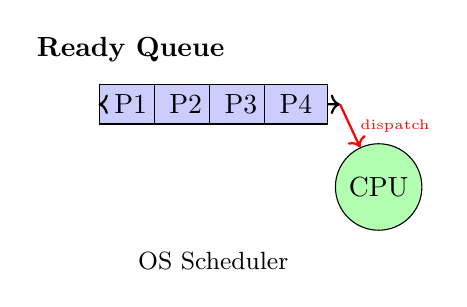
\begin{tikzpicture}[scale=0.7,
        proc/.style={rectangle, draw, minimum width=0.8cm, minimum height=0.5cm, fill=blue!20}]

        \node at (0,3) {\textbf{Ready Queue}};

        % Ready queue
        \node[proc] (p1) at (0,2) {P1};
        \node[proc] (p2) at (1,2) {P2};
        \node[proc] (p3) at (2,2) {P3};
        \node[proc] (p4) at (3,2) {P4};

        \draw[->, thick] (-0.5,2) -- (p1);
        \draw[->, thick] (p4) -- (3.8,2);

        % CPU
        \node[circle, draw, fill=green!30, minimum size=1cm] (cpu) at (4.5,0.5) {CPU};

        \draw[->, thick, red] (3.8,2) -- (cpu) node[midway,right] {\tiny dispatch};

        \node[below] at (1.5,-0.5) {\small OS Scheduler};
      \end{tikzpicture}
    \end{column}
  \end{columns}
\end{frame}

\begin{frame}{Queues in Networking}
  \begin{block}{Network Routers and Switches}
    \begin{itemize}
      \item Incoming packets queued before processing
      \item Multiple queues for Quality of Service (QoS)
      \item Different priority levels (voice, video, data)
      \item Scheduling algorithms: WFQ (Weighted Fair Queuing), Priority Queuing
    \end{itemize}
  \end{block}

  \vspace{0.3cm}

  \begin{columns}
    \begin{column}{0.48\textwidth}
      \begin{exampleblock}{Packet Queue Types}
        \begin{itemize}
          \item High priority: VoIP, video conferencing
          \item Medium priority: streaming video
          \item Best effort: web browsing, email
        \end{itemize}
      \end{exampleblock}
    \end{column}
    \begin{column}{0.48\textwidth}
      \begin{alertblock}{Queue Management}
        \begin{itemize}
          \item Drop-tail: drop when full
          \item Random Early Detection (RED)
          \item Token bucket rate limiting
        \end{itemize}
      \end{alertblock}
    \end{column}
  \end{columns}
\end{frame}

%----------------------------------------------------------------------------------------
%    COMPLEXITY ANALYSIS
%----------------------------------------------------------------------------------------
\section{Complexity Analysis}

\begin{frame}{Time and Space Complexity}
  \begin{center}
    \begin{tabular}{l|c|c|c|c}
      \toprule
      \textbf{Structure} & \textbf{Enqueue} & \textbf{Dequeue} & \textbf{Peek} & \textbf{Space} \\
      \midrule
      Queue (Array) & O(1) amortized & O(1) & O(1) & O(n) \\
      Queue (Linked List) & O(1) & O(1) & O(1) & O(n) + pointers \\
      Circular Queue & O(1) & O(1) & O(1) & O(capacity) \\
      Deque & O(1) & O(1) & O(1) & O(n) \\
      Priority Queue (Heap) & O(log n) & O(log n) & O(1) & O(n) \\
      \bottomrule
    \end{tabular}
  \end{center}

  \vspace{0.5cm}

  \begin{block}{Special Cases}
    \begin{itemize}
      \item For bounded integer priorities: Use bucket queues for O(1) operations
      \item For monotonic priorities: Consider monotonic queue optimization
      \item For small fixed priorities: Array of queues (one per priority level)
    \end{itemize}
  \end{block}
\end{frame}

%----------------------------------------------------------------------------------------
%    COMPARISON
%----------------------------------------------------------------------------------------
\section{Queue vs Stack}

\begin{frame}{Queue vs Stack Comparison}
  \begin{center}
    \begin{tabular}{l|c|c}
      \toprule
      \textbf{Property} & \textbf{Queue} & \textbf{Stack} \\
      \midrule
      Principle & FIFO (First In, First Out) & LIFO (Last In, First Out) \\
      Insert & Rear (enqueue) & Top (push) \\
      Remove & Front (dequeue) & Top (pop) \\
      Real-world & Waiting line & Plate stack \\
      Use case & Scheduling & Recursion, undo \\
      \bottomrule
    \end{tabular}
  \end{center}

  \vspace{0.5cm}

  \begin{columns}
    \begin{column}{0.48\textwidth}
      \begin{block}{Queue Applications}
        \begin{itemize}
          \item Breadth-First Search (BFS)
          \item Task scheduling
          \item Buffering
          \item Order processing
        \end{itemize}
      \end{block}
    \end{column}
    \begin{column}{0.48\textwidth}
      \begin{block}{Stack Applications}
        \begin{itemize}
          \item Depth-First Search (DFS)
          \item Expression evaluation
          \item Function calls
          \item Undo operations
        \end{itemize}
      \end{block}
    \end{column}
  \end{columns}
\end{frame}

%----------------------------------------------------------------------------------------
%    SUMMARY
%----------------------------------------------------------------------------------------
\section{Summary}

\begin{frame}{Key Takeaways}
  \begin{block}{Queue Fundamentals}
    \begin{itemize}
      \item FIFO data structure: First In, First Out
      \item Essential operations: enqueue (rear), dequeue (front)
      \item All basic operations are O(1) time complexity
    \end{itemize}
  \end{block}

  \begin{block}{Queue Variants}
    \begin{itemize}
      \item \textbf{Circular Queue}: Efficient space usage with wrap-around
      \item \textbf{Deque}: Double-ended queue for flexible insertion/deletion
      \item \textbf{Priority Queue}: Element ordering based on priority (heap-based)
    \end{itemize}
  \end{block}

  \begin{block}{Important Applications}
    \begin{itemize}
      \item Producer-consumer pattern and bounded buffers
      \item OS scheduling (CPU, I/O, process management)
      \item Network packet queuing and QoS
      \item BFS traversal and task scheduling
    \end{itemize}
  \end{block}
\end{frame}

\begin{frame}[plain]
  \begin{center}
    {\Huge Thank You!}

    \vspace{1cm}

    {\large Questions?}
  \end{center}
\end{frame}

\end{document}
